% Created 2020-05-29 Fri 13:54
% Intended LaTeX compiler: pdflatex
\documentclass[dvipdfmx]{article}
\usepackage[utf8]{inputenc}
\usepackage[T1]{fontenc}
\usepackage{graphicx}
\usepackage{grffile}
\usepackage{longtable}
\usepackage{wrapfig}
\usepackage{rotating}
\usepackage[normalem]{ulem}
\usepackage{amsmath}
\usepackage{textcomp}
\usepackage{amssymb}
\usepackage{capt-of}
\usepackage{hyperref}
\usepackage{minted}
\usepackage[utf8]{inputenc} % allow utf-8 input
\usepackage[T1]{fontenc}    % use 8-bit T1 fonts
\usepackage{hyperref}       % hyperlinks
\usepackage{url}            % simple URL typesetting
\usepackage{booktabs}       % professional-quality tables
\usepackage{amsfonts}       % blackboard math symbols
\usepackage{nicefrac}       % compact symbols for 1/2, etc.
\usepackage{microtype}      % microtypography
\usepackage{graphicx}
\usepackage[style=ieee, backend=biber, citestyle=numeric,natbib=true, sortlocale=en-US, sortcites]{biblatex}
\author{MokkeMeguru}
\date{\textit{<2020-05-29 Fri>} \today}
\title{Flow-based Model with Oxford flower 102 dataset}
\begin{document}

\maketitle
\tableofcontents


\section{Flow-based Model を使って、カラー画像を学習してみる}
\label{sec:orgabd025f}
Flow-based Model は逆関数のある深層学習モデル、というちょっと変わったモデルです。\\
このモデルは GANs や VAE を始めとする生成モデルの仲間に含められることが多く、実際に画像生成分野を中心に研究が進められています。\\

今回は Flow-based Model を用いて Oxford flower102 dataset という画像のデータセットを学習、何らかの画像を生成してみます。\\
\section{生成モデルと Flow-based Model}
\label{sec:org2d99bd0}
簡単に、この系統のモデルで出てくる要素は、 \textbf{画像} , \textbf{モデル} , \textbf{潜在表現} の3つです。\\

\begin{itemize}
\item 画像\\
画像とは実画像であったり生成画像であったり、人間が視認できるアレです。\\
\item モデル\\
何かから画像を生成したり、画像の意味を解釈して行列やベクトルといったもの(すぐ後に出てくる潜在表現)にしたりする機能を持った、 \textbf{箱} です。小麦を突っ込んだらパンが出てくるみたいな気持ちで見て下さい。\\
\item 潜在表現\\
ベクトルや行列の形で表される、人間が視認してもちょっとわからないけど、数学や統計の目で見ると画像などの性質を読み取ることの出来るものです。潜在表現は例えば勾配法などの数学・統計的手法を用いて操作することが容易になっています。\\
Flow-based Model や VAE は画像から潜在表現を作れます。そのため、画像から潜在表現を獲得、潜在表現を上手いこと調節して画像を再生成することで、イケメンが美少女になったりします。\\
\end{itemize}
\subsection{Flow-based Model の立ち位置}
\label{sec:orgd6a1e54}
Flow-based Model は VAE や GANs と比べて、画像から潜在表現をきっちり作れることが、特徴の1つです。この性質から、ちゃんとデータを与えて学習を行うと、そこそこに良い画像が生成できます。とはいえ GANs の方がモリモリ研究が進んでいるので、今の所 GANs のフィールドではそんなに勝てていません 。\\

\begin{center}
\begin{tabular}{llll}
\hline
 & 画像から潜在表現を作れるか & モデルの大きさ(パラメータ数) & 訓練時間\\
\hline
VAEs & 近似的に作れる & そこそこにでかい & 短\textasciitilde{}並\\
GANs & 作れない & でかい & 長・安定しない\\
Flow-based & 作れる & 小さい & 短\\
\hline
\end{tabular}

\end{center}
\section{今回作る Flow-based Model の概要}
\label{sec:orgb0e622f}
\subsection{まずは式で解釈する}
\label{sec:orgb4cbd1f}
\(x\) を画像、 \(f\) をモデル、 \(z\) を潜在表現とします。すると、Flow-based Model は次の式で表すことが出来ます。めっちゃシンプル。\\

\begin{eqnarray}
z = f(x) \ (\text{in training})\\
x = f^{-1}(z) \ (\text{in generating})
\end{eqnarray}

次に目的関数ですが、実際の画像 \(x\) の確率 \(p_X\) を高くする (つまり実際の画像が沢山生成できるようにする)、という意味を持っています。 \(p_X\)  はそのまま計算させることが難しいので、 モデル \(f\) を使って \(p_Z (z = f(x))\) とします。するとここの過程は変数変換 (ref. 極座標変換) なので、ヤコビアン \(J_f\) をくっつける必要があります。そのまま対数化すると下の式になります。\\

\begin{eqnarray}
p_X(x) = p_Z(z = f(x))|J_f|\\
log p_X(x) = \log(p_Z(z = f(x))) + \log |J_f|
\end{eqnarray}

\subsection{モデルの概要図}
\label{sec:org1578a39}
モデルはちょっと中身が複雑になっています。この Architecture が今の所 Flow-based Model の基本的な型になっています(ref. Glow, RealNVP, Flow++ etc.).\\
H, W, C はそれぞれ処理している行列の次元数を示しており、例えば image では H (height) x W (width) x C (channel) になっています。\\

この図を見ると、image から z へ一直線に流れる線と、 z\textsubscript{aux} というよくわからないものへ流れる線がわかります。 z\textsubscript{aux} というのは、 image から z へ処理していく中で、「もう  z とみなしちゃっていいでしょ」枠の行列です。これを設けることで、計算コストを抑えることが出来る他、 image から z へ流れの中で、画像の局所的な特徴を掴む部分 → 画像の全体的な特徴を掴む部分 と処理が行くようになります。\\

Squeezing やら Actnorm やら Inv1x1Conv, Affine Coupling あたりの話は、\href{https://qiita.com/exp/items/4f562ec788f2ac5241dc}{この辺りの要約} か \href{https://mokkemeguru.github.io/TFGENZOO/TFGENZOO.html}{ライブラリの実装ドキュメント} を見て下さい。\\
\begin{center}
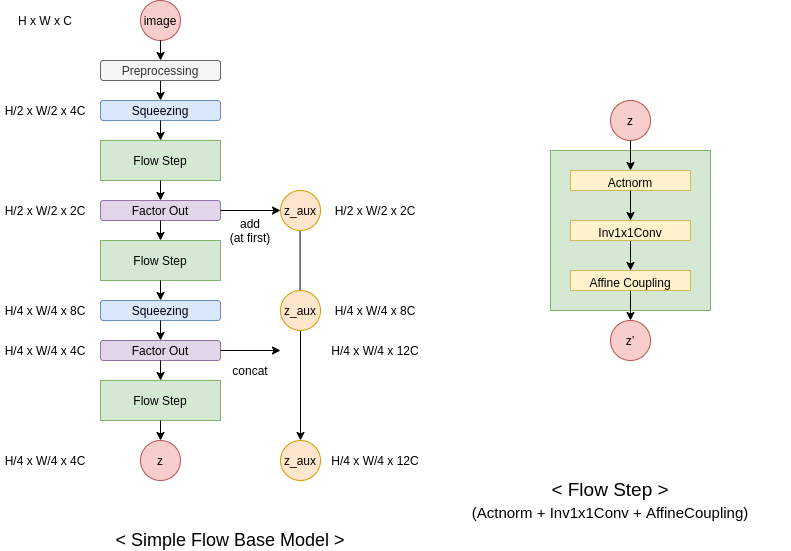
\includegraphics[width=\linewidth]{./simple_flow_image.png}
\end{center}
\section{Oxford flower102 データセットについて}
\label{sec:org194c07f}
Oxford flower102 データセットは flower の名前の通り、花の画像のデータセットです。内訳は下のテーブルになっていて、画像サイズは統一されていません。実験では計算機的問題から 48 x 48 にしています。データの前処理なんかは \href{https://github.com/MokkeMeguru/TFGENZOO\_EXAMPLE/blob/master/datasets/load\_flower.py}{こちら} を見て下さい (画像の data augumentation や前処理は素人なので、追加したほうが良い内容など教えて頂ければ幸いです)。このデータセットは元々クラス分類のためのデータセットなので近年の \textbf{でかいデータセット} + \textbf{潤沢な計算資源}  みたいなケースに比べるとかなり厳しい問題設定になっています。\\

\begin{center}
\begin{tabular}{lr}
\hline
 & 枚数\\
\hline
train & 1020\\
valid & 1020\\
test & 6149\\
\hline
\end{tabular}

\end{center}

\section{実際にコードを動かす}
\label{sec:orgaad07b5}
コードそのものは \href{https://github.com/MokkeMeguru/TFGENZOO\_EXAMPLE}{こちら} にあります。実行はこんな感じで出来ます。\\
\texttt{python glow.py} 以降はオプションで、 Facebook の \href{https://hydra.cc/}{hydra} というツールでパースさせています。より詳しいオプションが見たい場合は、 \texttt{python glow.py -{}-help} としてみて下さい。\\
\begin{minted}[frame=lines,linenos=true]{shell}
docker-compose build
docker-compose up -d
docker-compose exec tfgenzoo /bin/bash
tmux
python glow.py dataset=flower model.K=24 batch_sizes.0=32 batch_sizes.1=128 batch_sizes.2=128 epochs=512
\end{minted}

尚私の行なったGPU環境は、Quadro P6000 x 1 (4 hour) でした。GCE の無料枠か、Colab (頑張れば) で動くと思います。\\
\section{結果の観察}
\label{sec:org84edff5}
outputs/<date>/<time>/ 以下に生成されたモデル、ログが出力されます。Tensorboard を用いているので、こいつを使って可視化します。\\
まずは損失関数から。この損失関数は、先述の通り、実際の画像に高い確率を割り当てられたか、の結果になっており、上手いこと変形して最小化の形になっています。形を見ると大分綺麗に損失が下がっていることがわかると思います。尚、損失はまだまだ下がりそうなのに訓練していないのは、計算資源的事情です。\\
\begin{center}
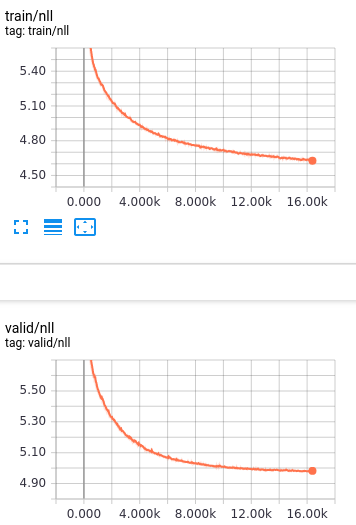
\includegraphics[width=0.5\linewidth]{./loss.png}
\end{center}

\subsection{生成画像の観察}
\label{sec:orgfbecd76}
次に生成画像を数 epoch ごとに見てみてます。\\

\begin{itemize}
\item 25 epoch\\
まだテクスチャ的な画像しか見えません。\\
\end{itemize}
\begin{center}
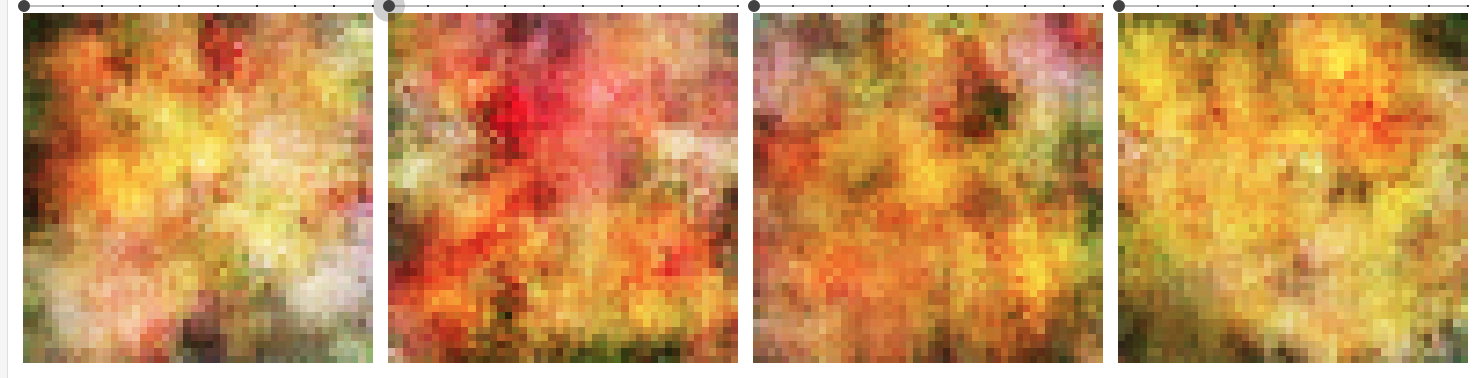
\includegraphics[width=0.75\linewidth]{./25epoch.png}
\end{center}

\begin{itemize}
\item 200 epoch\\
なんとなく周りは葉っぱにしたい気持ちが見えてきます。\\
\end{itemize}
\begin{center}
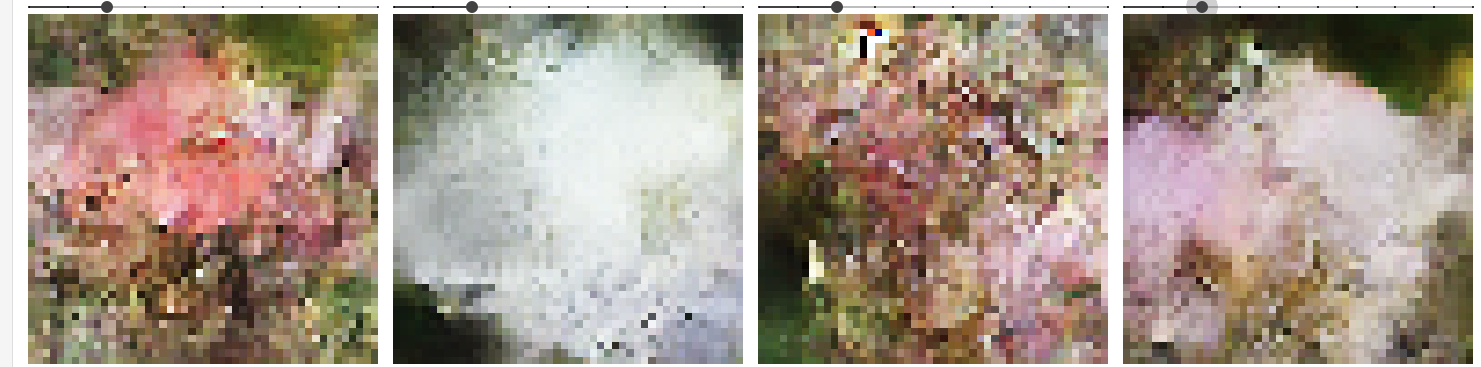
\includegraphics[width=0.75\linewidth]{./200epoch.png}
\end{center}

\begin{itemize}
\item 300 epoch\\
2番目あたりは大分それっぽい画像(解像度がアレ)になっています。\\
\end{itemize}
\begin{center}
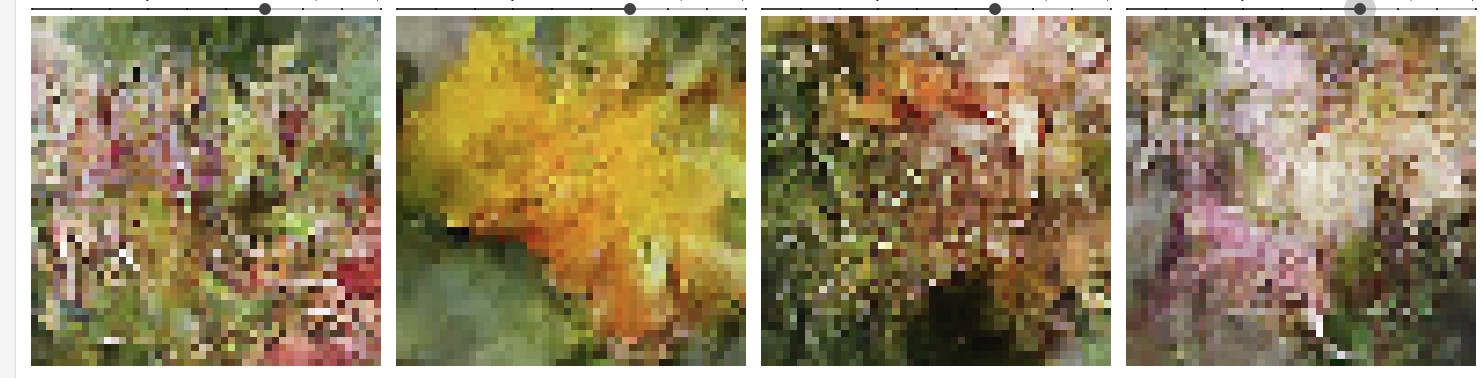
\includegraphics[width=0.75\linewidth]{./300epoch.png}
\end{center}

\begin{itemize}
\item 400 epoch\\
花弁と雌しべの領域的違いが見えてきました。\\
\end{itemize}
\begin{center}
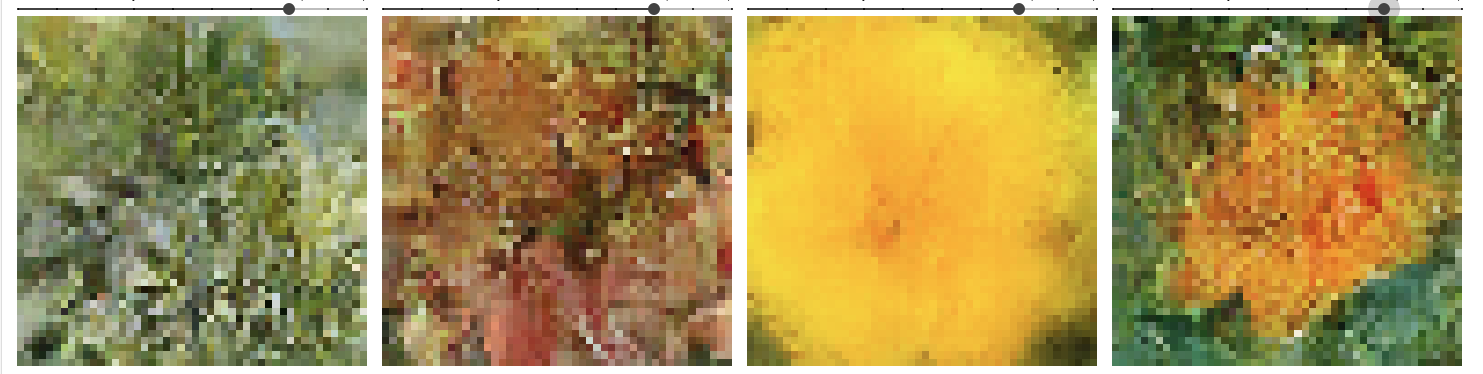
\includegraphics[width=0.75\linewidth]{./400epoch.png}
\end{center}

\begin{itemize}
\item 512 epoch\\
葉っぱと花の領域がかなりはっきり見分けがつくようになっています。が花の中の方はまだまだです。\\
\end{itemize}
\begin{center}
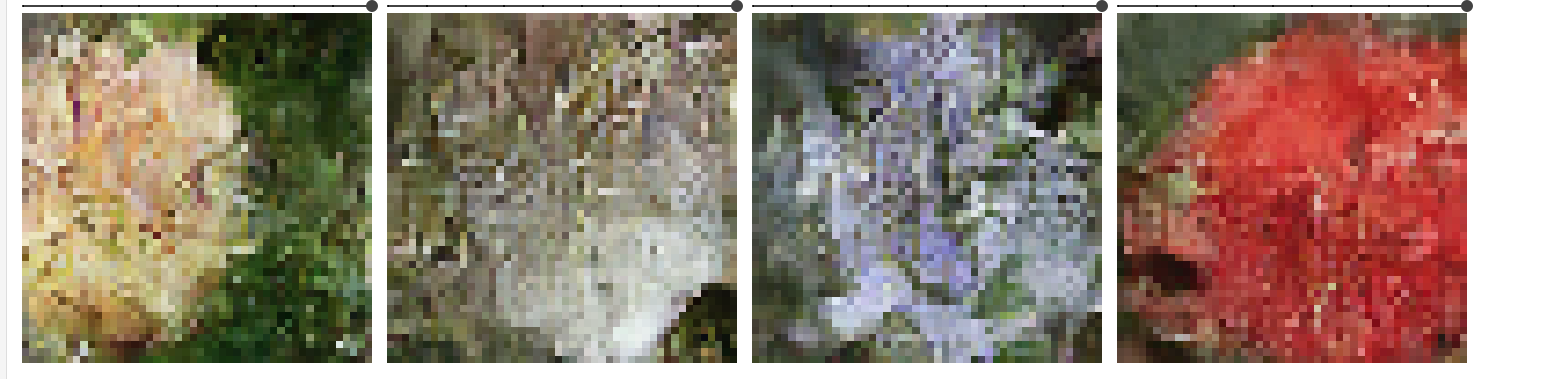
\includegraphics[width=0.8\linewidth]{./512epoch.png}
\end{center}

\subsection{再構成画像の観察}
\label{sec:orge3893d0}
そしてこちらは GANs と比較できないのであんまり注目されない部分ですが、再構成画像 (画像を潜在表現にして、もう一度画像にする)の結果も見てみます。\\

\begin{itemize}
\item 25 epoch\\
驚くべきことに学習初期は逆関数が正しく求まらず、きちんとした再構成画像が出てきません。\\
\begin{center}
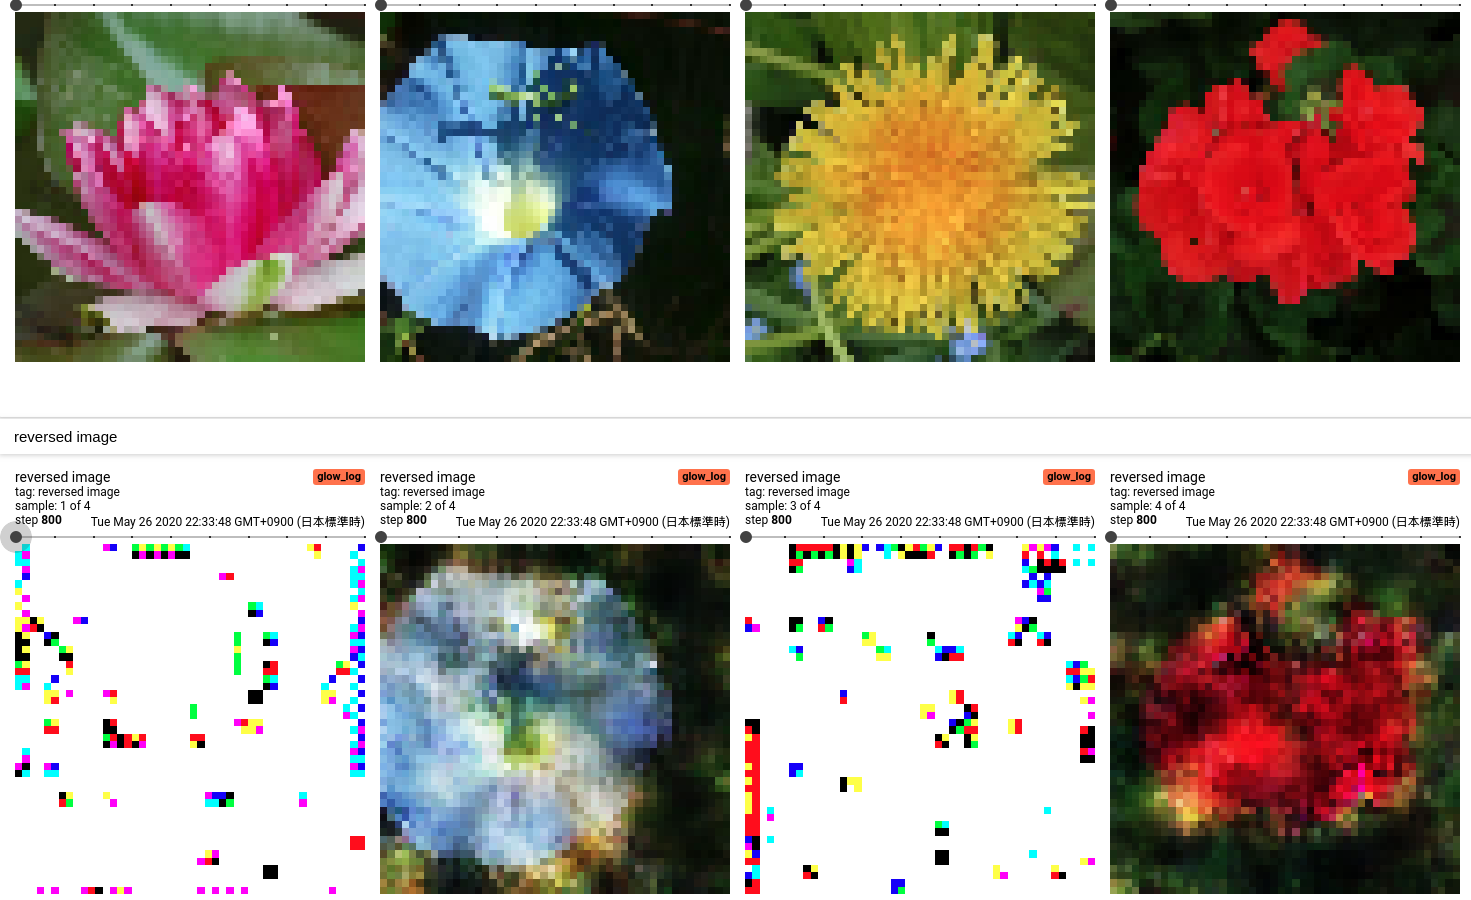
\includegraphics[width=0.8\linewidth]{./re25epoch.png}
\end{center}
\item 200 epoch\\
rgb = [0, 0, 0] の飛んだ値が出てきています。rgb の範囲的に [0, 1] ([0, 255])で値をクリッピングしているので、つまり白い部分は 値が0以下になってしまっていることを示しています。\\
\begin{center}
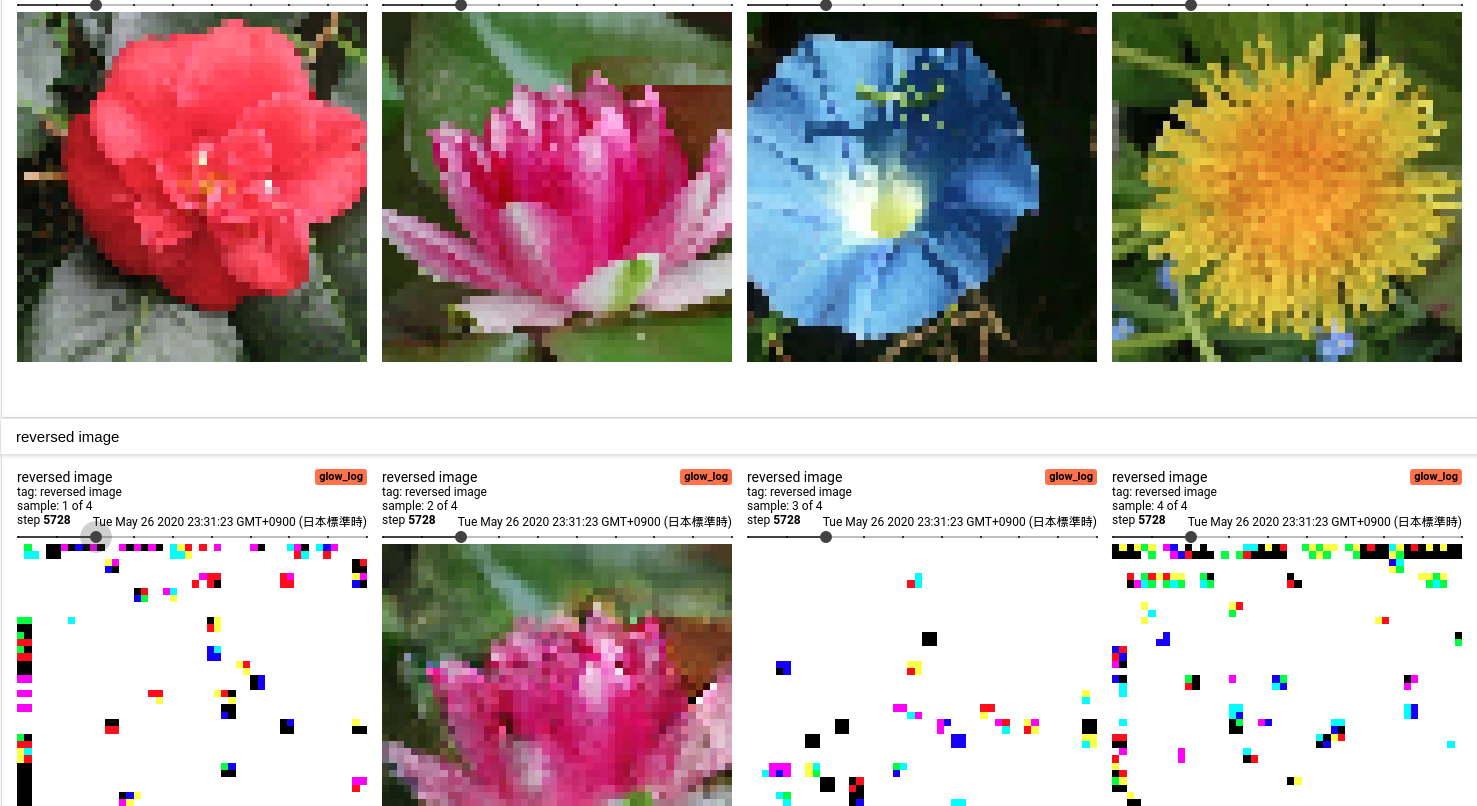
\includegraphics[width=0.8\linewidth]{./re200epoch.png}
\end{center}
\item 300 epoch\\
面白いことに、4枚目の画像は一部だけ正しい再構成画像が出来ているという不思議なことになっています。これは VAE や GANs などに比べてもかなり異質な特徴であると言えます。\\
\begin{center}
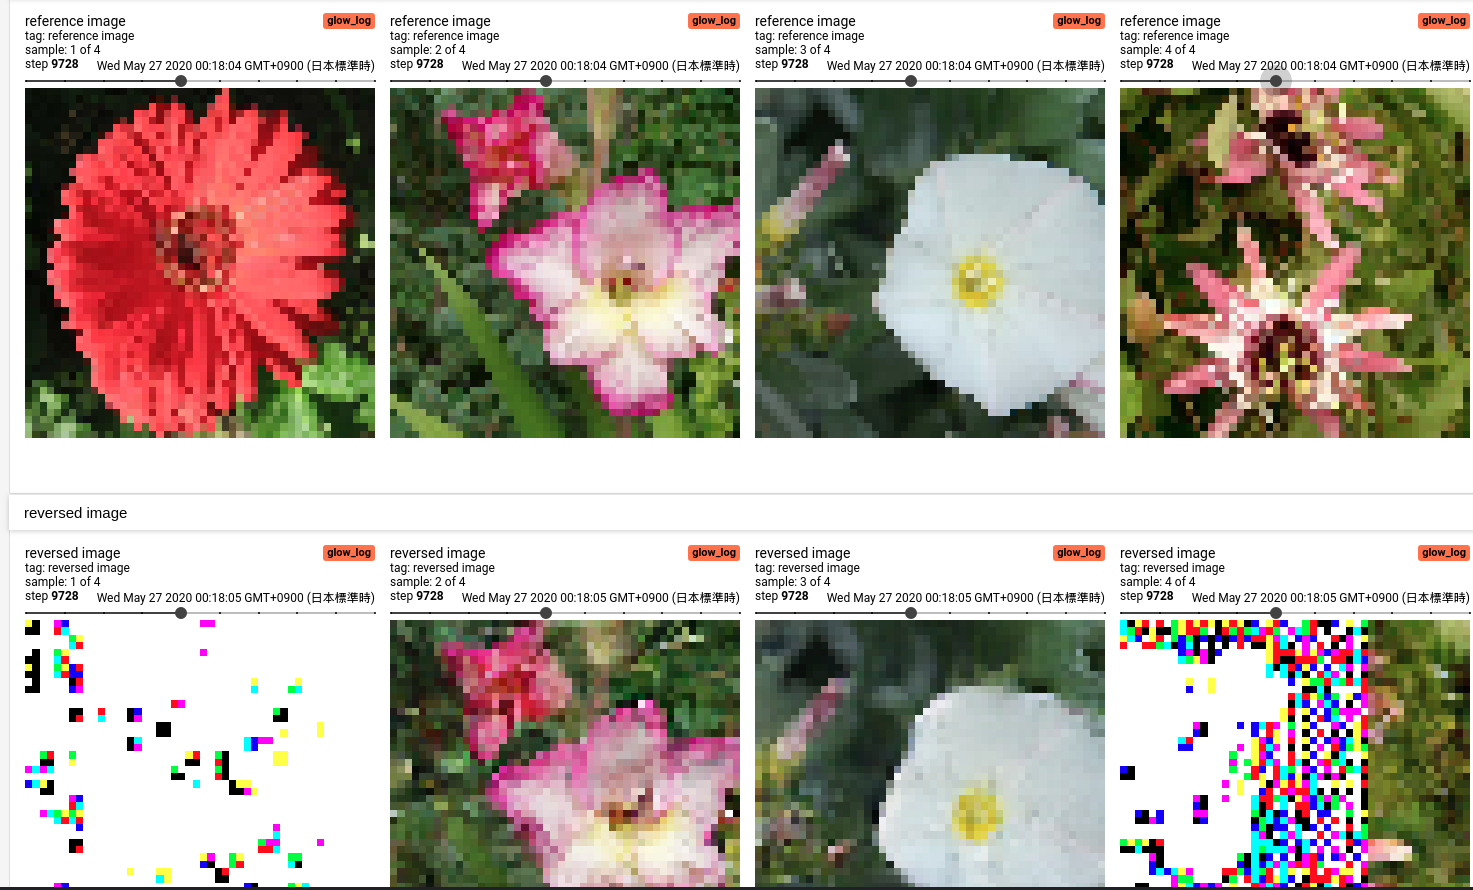
\includegraphics[width=0.8\linewidth]{./re300epoch.png}
\end{center}
\item 400 epoch\\
400 epoch になってもこの特徴は残っています。但し、上手く行っているものはきちんと再構成が出来ていることを確認できます。\\
\begin{center}
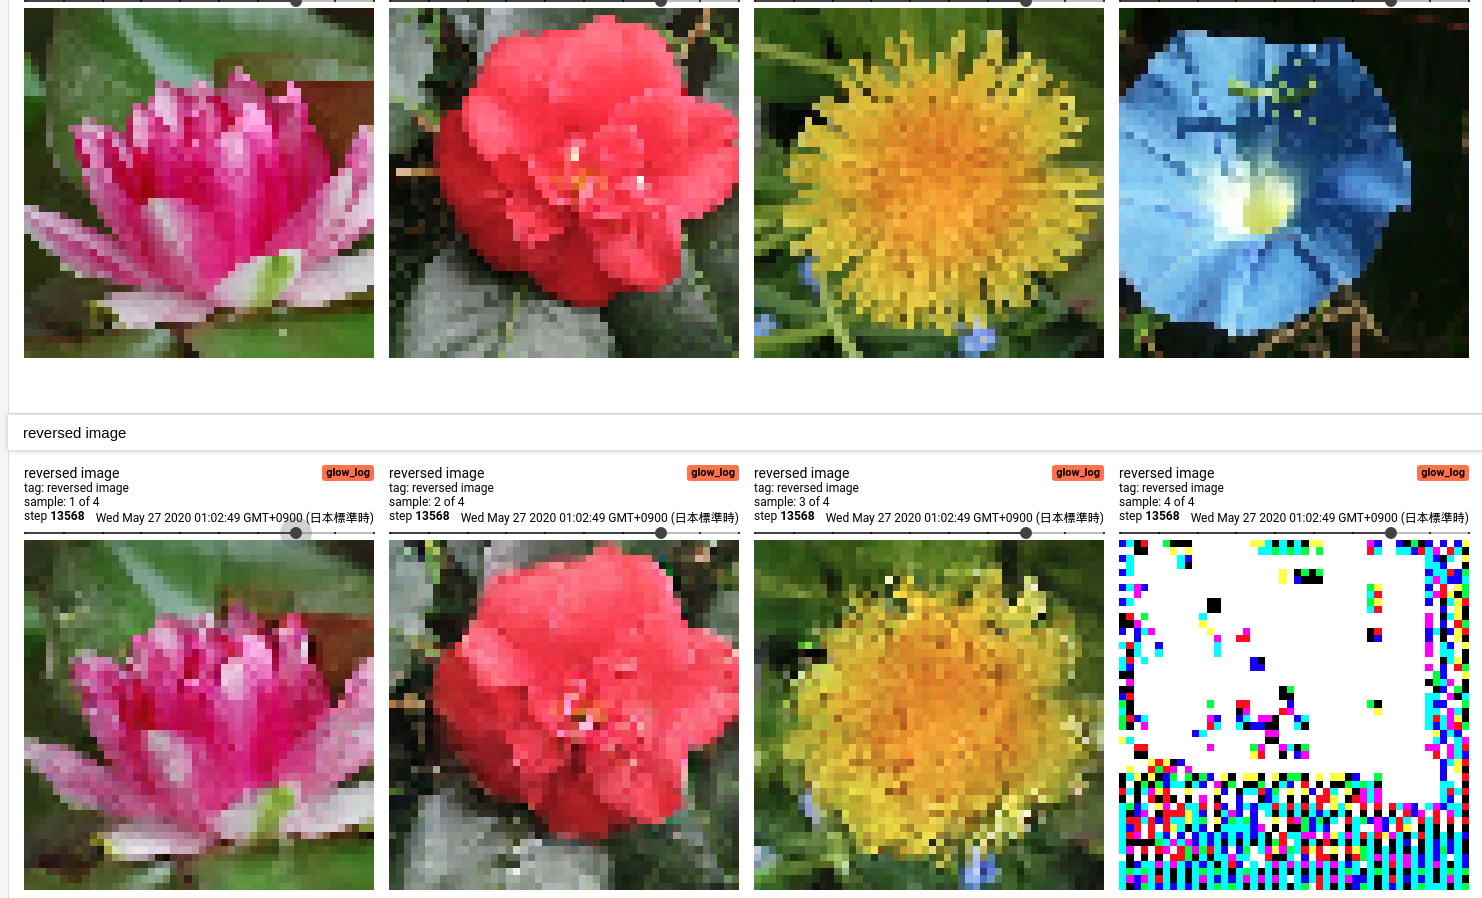
\includegraphics[width=0.8\linewidth]{./re400epoch.png}
\end{center}
\item 512 epoch\\
 この当たりになると、流石に飛んだ値は出なくなっているようです。再構成としても完全一致ではないですが、良いものができているような気がします。\\
\begin{center}
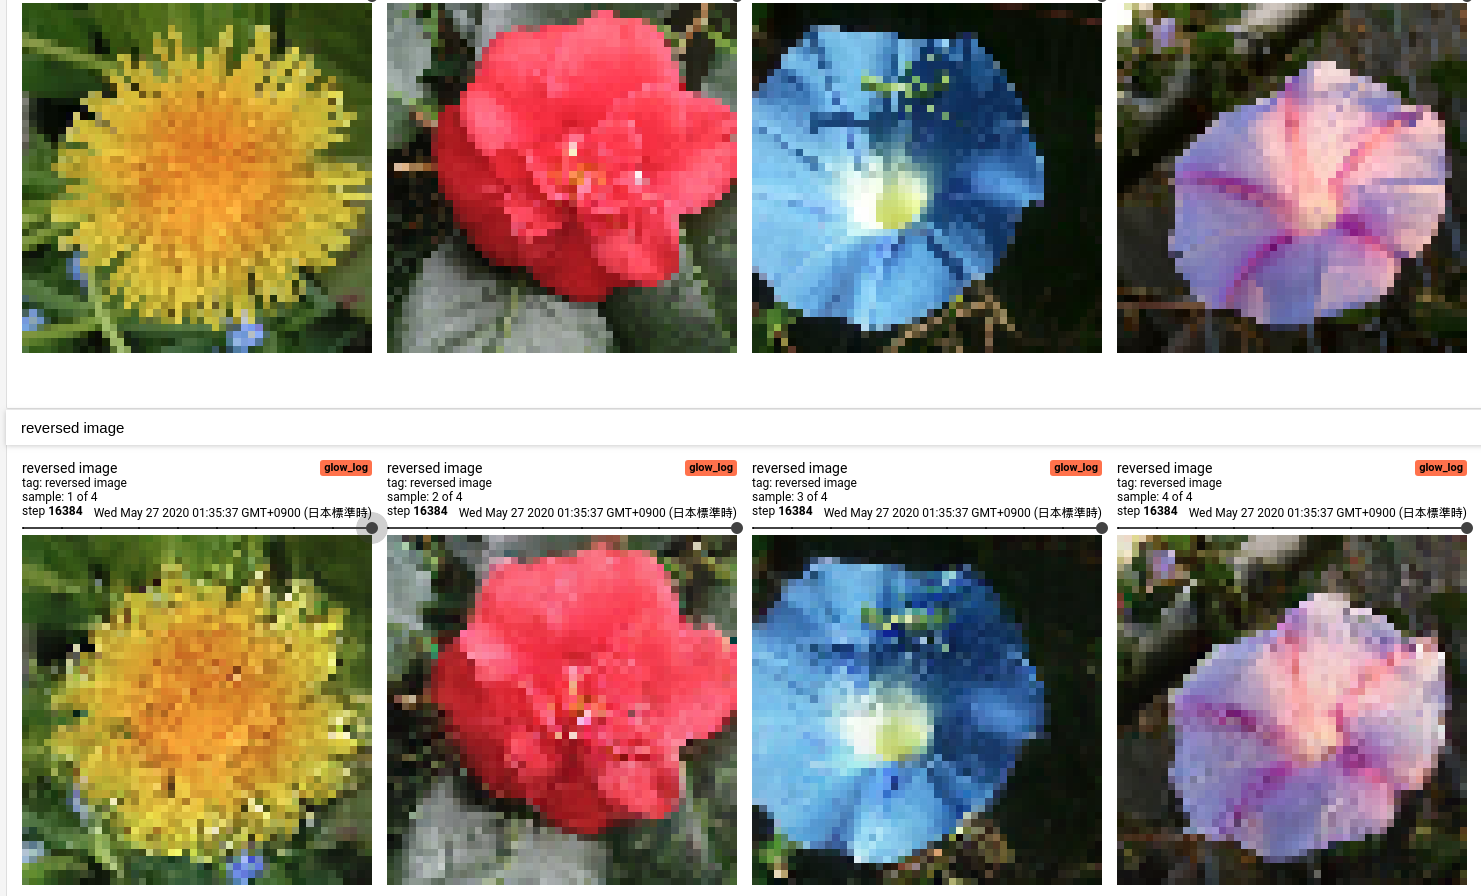
\includegraphics[width=.9\linewidth]{./re512epoch.png}
\end{center}
\end{itemize}
\section{考察}
\label{sec:org8e87b73}
\subsection{生成力が弱くない?}
\label{sec:org575711b}
計算資源的問題とデータ的問題を抜きにして話すならば、Data Augumentation の知見が不足していることや、内部で用いている AffineCoupling というレイヤーについて問題があると考えています。AffineCoupling レイヤーは \href{https://arxiv.org/pdf/1902.00275.pdf}{Flow++} という最近出てきたネットワークでより良いバージョンが提案されており、ここを更新することでもう少し生成力を高められると思います。(とはいえこのレイヤーは実装がものすごく大変です。具体的には深層学習モデル中に、累積分布関数を導入します)\\

\subsection{生成画像がちょっとボケてない?}
\label{sec:org31fdf4e}
生成画像がボケる理由は、MLE (maximum likelihood estimation)という最適化手法を取っているためです。これは GANs の Adversarial Training と比較されることがしばしばあり、前者は画像がボケやすくなることが、後者は mode collapse という生成画像が似たようなものしか出てこないことが指摘されています。\\

直感的に MLE の画像がボケる理由としては、なんとなく実際の画像っぽい画像にも高い確率を与えてしまうことにあります。潜在表現は似た画像は同じような潜在表現を持つため、実際の画像に高い確率を与えてしまうと、自然とそれっぽい (ちょっとボケた) 画像も高い確率が与えられてしまいます。\\

\subsection{再構成画像おかしくない?}
\label{sec:orgaf7ab16}
再構成画像、おかしいですねぇ。ただ丸め誤差や、内部で用いている対数関数や指数関数などが悪さをしているのではないかと考えています。\\
また、Flow-based Model は画像の rgb が [0, 255] の離散値を \textbf{ノイズをかけて} 連続値にしているという理由もあると考えています。\\
\section{GANs is better than Flow}
\label{sec:orge4ae2c0}
よく言われるものとして、やっぱ GANs が最強っていうのがあります。実際に Flow-based Model の研究のかなりは vs GANs を意識したものを書いています。\\
とはいえ、Flow-based Modelは、\href{https://arxiv.org/abs/1907.02392}{一部のスタイル変換} (ICLR でニッチな需要だねw なんて言われてますが、グリザイユ画法という立派な絵画手法であったりします)や、 \href{https://openreview.net/forum?id=SJxE8erKDH}{画像とテキストを関連付けるタスク} (画像の潜在表現と文の潜在表現をエイヤッと Flow-based Model でくっつけます) なんかで強力な \textbf{力} を見せています。またモデルパラメータや計算資源使用量も比較的少なくても上手く行くようになっているので、面白い分野ではあるんじゃないかなと思います。\\

\begin{figure}[htbp]
\centering
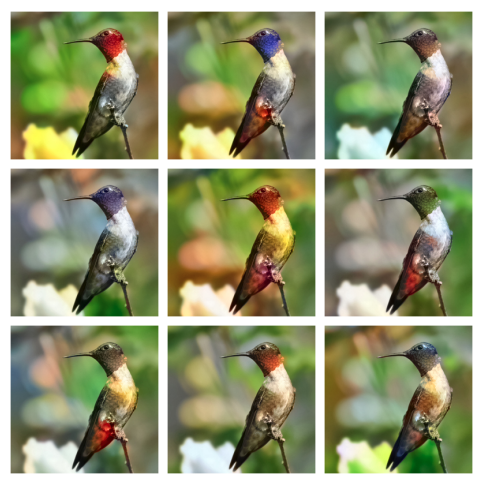
\includegraphics[width=10cm]{./cinn.png}
\caption{GUIDED IMAGE GENERATION WITH CONDITIONAL INVERTIBLE NEURAL NETWORKS}
\end{figure}

\begin{figure}[htbp]
\centering
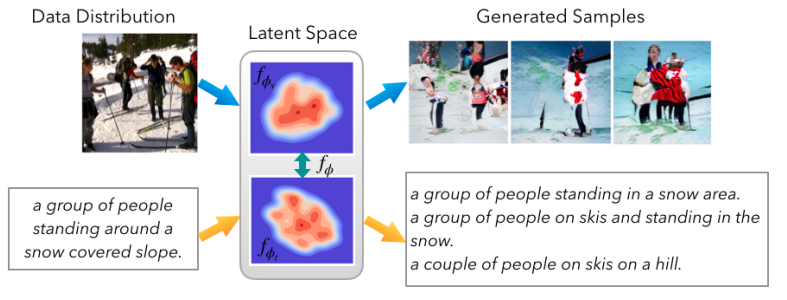
\includegraphics[width=.9\linewidth]{./connect.png}
\caption{Latent Normalizing Flows for Many-to-Many Cross-Domain Mappings}
\end{figure}
\section{ライブラリの話: TFGENZOO}
\label{sec:org8fec0a0}
\subsection{TFGENZOO について}
\label{sec:orge87a042}
こいつは今インターンシップを中心に開発を進めている Flow-based Model 系の生成モデルの作成を支援するライブラリです。 Tensorflow 2.x 系の上に作られており、数式とモデルの実装が出来るだけ近くなる (関連がわかりやすくなる) ように注意して作っています。使い方やドキュメントは \href{https://github.com/MokkeMeguru/TFGENZO}{レポジトリ} や \href{https://github.com/MokkeMeguru/TFGENZOO\_EXAMPLE}{Example}, あるいは \href{https://github.com/MokkeMeguru/TFGENZOO/issues/new}{Issue} を参照して下さい。\\
\subsection{今回の実装の詳しい話}
\label{sec:org5237c70}
実装の詳しい話をすると、\href{https://github.com/MokkeMeguru/TFGENZOO\_EXAMPLE/blob/c63288de6ab64002c5986c1d6dadbd1bb0f83df0/models/glow.py}{こちら} がモデルファイルになっています。基本的には概要図のとおりですが、注意する点として、次の部分があります。\\

\begin{minted}[frame=lines,linenos=true]{python}
class Glow(Model):
    def __init__(self, hparams: Dict):
        super().__init__()
        self.model_params = hparams["model"]
        K = self.model_params["K"]
        L = self.model_params["L"]
        conditional = self.model_params["conditional"]
        flows = []
        flows.append(LogitifyImage())
        for layer in range(L):

            # Squeezing Layer
            if layer == 0:
                flows.append(Squeezing(with_zaux=False)) # <--- !!!
            else:
                flows.append(Squeezing(with_zaux=True))
            fml = []

            # build flow module layer
            for k in range(K):
                fml.append(Actnorm())
                fml.append(Inv1x1Conv())
                scale_shift_net = ShallowResNet(
                    width=self.model_params["hidden_width"])
                fml.append(AffineCoupling(
                    mask_type=AffineCouplingMask.ChannelWise,
                    scale_shift_net=scale_shift_net))
            flows.append(FlowModule(fml))

            # Factor Out Layer
            if layer == 0:
                flows.append(
                    FactorOut(with_zaux=False # <--- !!!
                              conditional=conditional))
            elif layer != L - 1:
                flows.append(
                    FactorOut(with_zaux=True,
                              conditional=conditional))

        self.flows = flows
\end{minted}

with\textsubscript{zaux} というのは、モデルの概要図的に、「横に z\textsubscript{aux} が見えるか」 というフラグになっています。これは z\textsubscript{aux} が img → z の処理と同じように次元数を変えるために必要になっています。\\
\end{document}
